\documentclass{article}

\usepackage[T1]{fontenc} 
\usepackage[french]{babel}
\usepackage[utf8]{inputenc}
\usepackage{xskak}
\usepackage{subfig}
\usepackage[frenchkw]{algorithm2e}
\usepackage{graphicx}
\graphicspath{{./img/}}
\usepackage{amsmath, amssymb}
\usepackage[left=3cm,right=3cm,top=2cm,bottom=2cm]{geometry}
\usepackage{url}
\usepackage[linktocpage=true]{hyperref}
\usepackage{tikz}
\usepackage{float}

\title{Rapport de Projet : Amazons the game}
\author{Youri CHANCRIN, Théo DESCOMPS, Samuel KHALIFA, Jean-Baptiste MARTINEZ}
\date{\today}

\makeatletter
\let\mytitle\@title
\let\myauthor\@author
\makeatother

\begin{document}

\begin{flushleft}

\thispagestyle{empty}

\includegraphics[width=0.2\textwidth]{enseirb-matmeca}
\graphicspath{{./img/}}

\vspace{\stretch{0.4}}

\hrulefill \\[2em]
\begin{center}
\textbf{\Huge \mytitle}\\[0.8em]
{\large Équipe : projetss6-amaz-19048}
\\[0.8em]
\end{center}
\hrulefill

\vspace{\stretch{0.6}}

{\large \textbf{Auteurs :} \myauthor}\\
\vspace{\stretch{0.2}}
{\large \textbf{Responsable de projet :} David Renault}\\
\vspace{\stretch{0.2}}
{\large \textbf{Enseignant référent :} Mihail Popov}

\vspace{\stretch{1}}

\begin{center}
  Première année, filière informatique\\
  Date : \today
\end{center}

\vspace{\stretch{1}}

\hfill Version actuelle du document : Finale

\end{flushleft}

\newpage

\tableofcontents

\newpage

\section{Présentation du sujet}
L'objectif de ce projet est la création d'un serveur de jeu et de clients pouvant faire des parties 
du jeu des amazons.

Le jeu des amazons est un jeu de plateau où deux joueurs s'affrontent en jouant tour à tour.
Ils disposent chacun de reines, qui ont des mêmes déplacements que les reines des échecs.
Durant son tour, un joueur bouge une de ses reines, puis tire une flêche depuis la position atteinte par la reine.
La flêche est lancée sur l'une des 8 directions cardinales et ne peux traverser de reines ou d'autres flêches.

Le premier joueur qui ne peut pas jouer un coup valide perd.

Pour répondre à ce besoin, nous avons suivis les spécifications du sujet,
mis en place une infrastructure client-serveur, et réalisé plusieurs clients 
capable de jouer une partie, et souvent la gagner.

\subsection{Spécifications du sujet}
Le sujet nous demandait d'implémenter un modèle client-serveur et nous a
contraint à utiliser la librairie GSL.

\subsubsection{Structure Client Serveur}

La structure client-serveur, autrement appelée "monolithe", permet de séparer
la responsabilité des joueurs et du jeu en lui même. Le serveur représente le jeu. Il organise le
déroulement du jeu, retransmet l'information d'un client $x$ aux autres clients et vérifie que tout coup joué est valide.

\subsubsection{Utilisation de GSL}

Il nous a été demandé de représenter le plateau de jeu comme un graphe.
Cela permet quelques folies pour implémenter moultes plateaux intéressant.
Dans les règles des échecs, une case aura au plus 8 voisins, cela veut dire que dans le graphe, un noeud aura au maximum 8 voisins, alors qu'un graphe fait au moins 25 noeuds.
Pour représenter ce graphe, il nous a été demandé de le représenter par sa matrice d'adjacence.
Plus exactement, on stocke la direction entre le sommet i et le sommet j dans la matrice d'adjacence comme montré dans la Figure \ref{fig:ex-matrice-adj}.
Pour stocker cette matrice, nous étions contraints d'utiliser la GNU Scientific Library (GSL).
Cette librairie permet le stockage et traitement de matrices optimisées autrement appelées \textit{matrices creuses}.
Il aurait peut-être été plus judicieux de stocker une liste d'adjacence directement, mais les matrices creuses sous format Compressed Sparse Row (CSR) peuvent s'apparenter à cela.

\begin{figure}[H]
	\centering
	\raisebox{-0.5\height}{
		\subfloat[][Un graphe 2x2]{
			\begin{tikzpicture}
				\begin{scope}[every node/.style={draw, circle}]
					\node (0)[draw, circle] at (0,0) {0};
					\node (1)[draw, circle] at (2,0) {1};
					\node (2)[draw, circle] at (0,-2) {2};
					\node (3)[draw, circle] at (2,-2) {3};
				\end{scope}
				\begin{scope}[every edge/.style={draw, very thick}]
					\path [-] (0) edge node {} (1);
					\path [-] (0) edge node {} (2);
					\path [-] (1) edge node {} (3);
					\path [-] (2) edge node {} (3);

				\end{scope}
			\end{tikzpicture}
		}
	}
	\hspace{2em}
	\raisebox{-0.25\height}{
		\subfloat[][Sa matrice d'adjacence]{
			$\begin{bmatrix}
					NO\_DIR & EAST    & SOUTH   & NO\_DIR \\
					WEST    & NO\_DIR & NO\_DIR & SOUTH   \\
					NORTH   & NO\_DIR & NO\_DIR & EAST    \\
					NO\_DIR & NORTH   & WEST    & NO\_DIR \\
				\end{bmatrix}$
		}
	}
	\caption{Exemple de graphe et sa représentation en matrice d'adjacence}
	\label{fig:ex-matrice-adj}
\end{figure}

Enfin, le sujet demandait à implémenter les plateaux présenté en figure \ref{fig:all-boards}

\begin{figure}[H]
	\centering
	\subfloat[][Plateau classique]{
		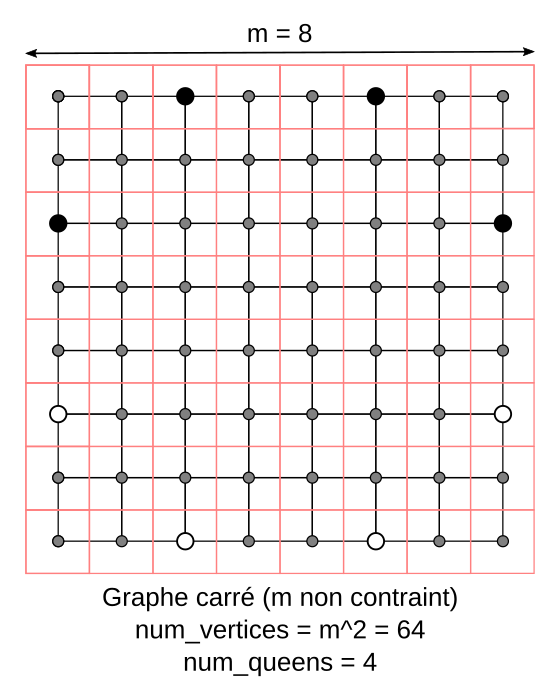
\includegraphics[width=0.3\linewidth]{classic_board}
	}
	\subfloat[][Plateau donut]{
		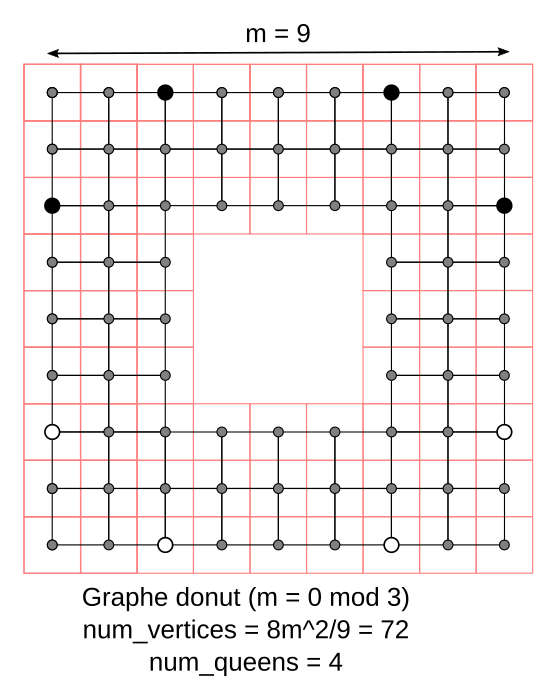
\includegraphics[width=0.3\linewidth]{donut_board}
	}

	\raisebox{-0.5\height}{
		\subfloat[][Plateau trèfle]{
			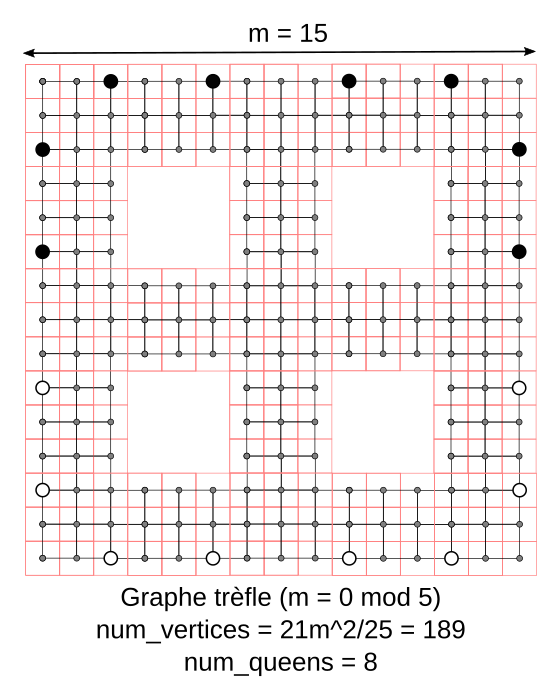
\includegraphics[width=0.3\linewidth]{clover_board}
		}
		\subfloat[][Plateau huit]{
			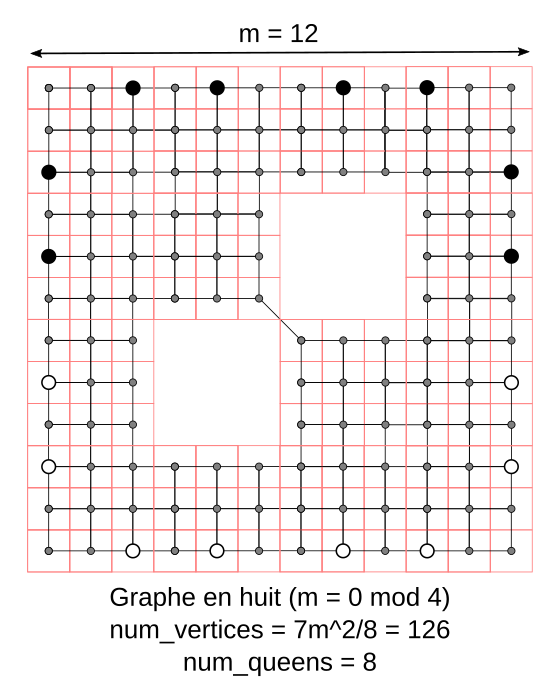
\includegraphics[width=0.3\linewidth]{eight_board}
		}
	}
	\caption{Les différents plateaux à implémenter et leurs graphes}
	\label{fig:all-boards}
\end{figure}

\subsubsection{Utilisation de libdl}

Chaque client devait être compilé en tant que librairie dynamique.
Le serveur devait lancer les clients en tant que librairies dynamiques ouvertes
au \textit{runtime} en utilisant la fonction \verb|dlopen| de la librairie \verb|libdl|

\section{Modèle Client-Serveur}
Le modèle client serveur implique deux choses.
Premièrement, il est nécessaire d'isoler les responsabilités entre le module client et le module serveur.
Secondement, il est nécessaire d'avoir une interface pour que les modules puissent communiquer.
Cette dernière est imposée par le sujet.

\subsection{Isolation des responsabilités}

Le serveur est responsable du lancement, du déroulement, ainsi que la terminaison de la partie.
Le client est responsable des coups qu'il joue lorsque le serveur lui demande de jouer, 
en l'informant du coup de son adversaire au tour précédent.

On remarque que les deux modules ont besoin de pouvoir garder en mémoire l'évolution d'une partie.
Le serveur en a besoin pour savoir si un joueur fait un coup invalide.
Les clients en ont besoin pour suivre une stratégie cohérente.

On décide de faire un troisième module nommé Common qui implémentera toutes les fonctionnalités communes 
aux clients et au serveur.

\subsection{Interface entre client et serveur}

Les clients doivent disposer de quatres fonctions.
\begin{itemize}
    \item \textbf{get\_player\_name()} : Retourne le nom du joueur.
    \item \textbf{initialize()} : Permet au joueur de se prépaprer pour la partie à venir.
    \item \textbf{play(coup\_precedent)} : Demande au joueur un coup, en fonction 
    du coup fait par son adversaire au tour précédent.
    \item \textbf{finalize()} : Permet au joueur de libérer les ressources allouées.
\end{itemize}

Cette interface établie une généricité entre tous les clients et permet de les faire s'affronter.
Cela rend possible la création d'une compétition pour établir quelle est 
la meilleur stratégie.

\section{Module Serveur}
Le serveur s'occupe de gérer une partie jouée par deux clients. 

D'une part, il s'occupe de l'isolation de la mémoire lors de l'initialisation.
D'autre part, il doit être capable de déterminer le gagnant de la partie.


\subsection{Isolation de la mémoire}
Le serveur copie les données d'initialisation de la partie pour chaque client.
Cela empêcherait un potentiel client malicieux de modifier la mémoire du serveur ou 
de son adversaire.
Dans le cas où les clients et le serveur seraient sur des machines séparées, 
la question ne se poserait pas et les clients seraient contraints
d'allouer eux-mêmes la mémoire pour cette tâche.

\subsection{Détermination du vainqueur}
Au fur et à mesure de la partie, le serveur reçoit les coups des deux joueurs.
Il applique les modifications engendrées par ces coups sur un plateau dont seul lui a l'accès.
Ce plateau est fourni par le module Common. Lorsque que le serveur obtient le coup 
du joueur courrant, il effectue un test à l'aide la fonction \textbf{is\_move\_legal()} de l'interface board.h.
S'il reçoit la valeur false, le joueur courrant à perdu, l'autre joueur est donc le vainqueur.

\section{Module Common}
Le module \verb|common| contient un ensemble de fonctionnalités qui sont 
utilisées à la fois par le serveur et par les clients. 

\subsection{Structures de données}
Le module \verb|common| dispose de plusieurs structures de données:
\begin{itemize}
    \item \textbf{array\_list} : Un tableau dynamique pouvant contenir n'importe quel objet.
    \item \textbf{position\_set} : Un ensemble de positions.
    \item \textbf{tree} : Un arbre d'objets quelconque.
    \item \textbf{zobrist\_hash} : Permet de \textit{hasher}\footnote{Un hash consiste à calculer un nombre le plus unique possible d'une structure de données quelconque} un plateau de jeu.
    \item \textbf{board} : Une représentation du plateu de jeu.
\end{itemize}

Ces structures offrent une diversité de complexités dont les clients 
peuvent se servir pour minimiser leurs temps d'éxecutions.

Les avoir à disposition de tous les clients simplifie le prototypage de nouvelles stratégies.
Par exemple, la structure \verb|tree| permet de modéliser un arbre des parties possibles pour les 
stratégies qui gardent en mémoire une prévision des prochains tours.

\subsection{Plateau de jeu}
Le plateau de jeu enveloppe le graphe fournit par GSL.
Ce-dernier étant dans un format optimisé, on a choisit de ne jamais 
le modifier car c'est une opération couteuse et complexe. Pour 
enregistrer les évolutions de la partie, nous avons décidé de stocker les
flèches posées sur la plateau comme un booléen indiquant si la case $c$ est bloquée par une flèche ou non.
Pour les reines, nous avons décidé de d'abord stocker la position des reines pour chaque joueur,
puis après quelques étapes de \emph{profilage} pour optimiser nos clients, nous avons rajouté
un autre moyen d'accéder aux reines sur le plateau.

\section{Module Client}
Un client doit retourner un coup à jouer lorsque le serveur lui demande.
Ce coup doit être valide, si cela est possible.

Tous les clients disposent des fonctions de l'interface imposées.
La différence principale se situe au niveau de la fonction \textbf{play()}.

\subsection{Client Random}
\subsection{Client Alphabeta}
\subsection{Client MCTS}

\section{Optimisations}
Durant le développement de nos différents clients, nous nous sommes rendus
compte que nous étions très limité par le temps de calcul. En effet,
la plupart de nos algorithmes n'étaient pas optimisés. Nous avons donc
eu recourt à du profilage

\subsection{Profilage et identification de zone critiques}
Après un premier appel au profileur \textit{gprof} montré dans la Figure \ref{fig:gprof-find-neighbors}
, nous voyons déjà une première zone critique, \verb|find_neighbor_in_direction|.

\begin{figure}[H]
	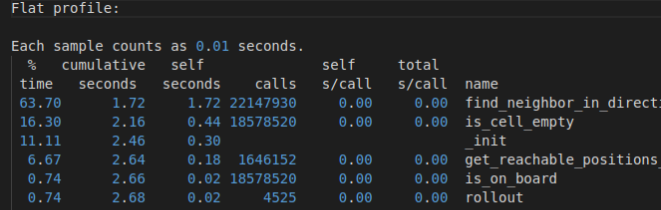
\includegraphics[width=\linewidth]{gprof_neighbors}
	\caption{Résultat du profileur \textit{gprof} après exécution d'une itération MCTS}
	\label{fig:gprof-find-neighbors}
\end{figure}

On remarque que la fonction \verb|find_neighbor_in_direction| nous mange
toute la puissance de calcul. Cette fonction est appelée plus de 22 millions de fois, elle 
occupe 63.70\% du temps CPU et la somme de la durée prise par tous ses appels est égale à 1.72 secondes, ce qui est gigantesque
pour une seule itération de MCTS. Au moment du \textit{profiling}, la fonction \verb|find_neighbor_in_direction| avait le fonctionnement défini
dans l'algorithme \ref{alg:find_neighbor_before}. Sa complexité était au moins de $O(nombre\_sommets)$ soit $O(n)$. Nous voudrions une complexité
$O(1)$ idéalement vu le nombre d'appels à cette fonction.

\begin{algorithm}
	\Entree{M: matrice d'adjacence, d: direction, i: $\mathbb{N} < nbre\_sommets$}
	\Deb{
		\PourTous{$0 \leq j < nbre\_sommets$}{
			\lSi{$M_{i,j} = dir$}{
				\Retour{j}
			}
		}
		\Retour{-1}\;
	}
	\caption{Algorithme peu efficace pour trouver le voisin dans une direction}
	\label{alg:find_neighbor_before}
\end{algorithm}

2 idées ont été implémentées pour améliorer cette méthode. Premièrement, on stocke le résultat
de l'algorithme dans un cache, donnant une complexité moyenne $O(1)$. Deuxièmement, la première approche
était très naïve, elle ne prenait pas en compte l'avantage du format CSR. En effet, avec le format CSR,
on peut tout simplement itérer sur les valeurs non zéros à la ligne $i$, ce qui équivaut à itérer sur tous
les voisins de $i$. Cette deuxième approche est de complexité $O(NUM\_DIRS)$, donc est aussi $O(1)$.
En fusionnant les deux approches, on peut obtenir l'algorithme \ref{alg:find_neighbor_opti} qui est très efficace
et prends avantage de nos structures de données.

\begin{algorithm}
	\Entree{M: matrice d'adjacence, d: direction, i: $\mathbb{N} < nbre\_sommets$}
	\Deb{
		\lSi{is\_neighbor\_cached(dir, i)}{
			\Retour{cached\_neighbor(dir, i)}
		}
		\PourCh{$j \in voisins(i)$}{
			\lSi{$M_{i,j} = dir$}{
				\Retour{j}
			}
		}
		\Retour{-1}\;
	}
	\caption{Algorithme peu efficace pour trouver le voisin dans une direction}
	\label{alg:find_neighbor_opti}
\end{algorithm}

Après application de ces résultats et un appel à \textit{gprof} affiché dans la Figure \ref{fig:gprof-empty-cell},
une nouvelle zone critique apparait: \emph{is\_cell\_empty}.
\begin{figure}[H]
	\centering
	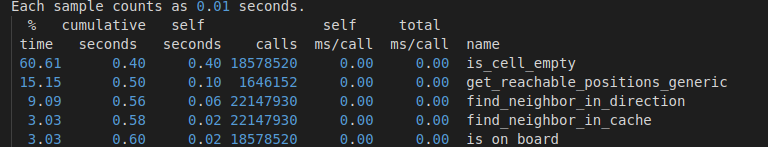
\includegraphics[width=\linewidth]{gprof_cell_empty}
	\captionsetup{justification=centering}
	\caption{Résultat du profileur \textit{gprof} après exécution d'une itération MCTS \\et optimisation \textit{find\_neighbor\_in\_direction}}
	\label{fig:gprof-empty-cell}
\end{figure}

Cette fois-ci, c'est \textit{is\_cell\_empty} qui occupe toutes les ressources CPU. La raison est simple,
nous stockons actuellement les positions des reines par joueur. Pour savoir si une case est vide,
il faut donc itérer sur toutes les reines de tous les joueurs pour savoir s'il y a une reine, et regarder s'il y a une flèche à cette position.
Là encore, nous avons un vilain $O(n)$ couplé à un nombre d'appels colossal. Cependant, la solution à ce problème
n'est pas si élégante que celle pour \textit{find\_neighbor\_in\_direction}. En effet,
nous devons dupliquer de l'information, car stocker les reines par joueur est intéressant pour d'autres algorithmes.
Nous avons donc décidé d'avoir une redondance de l'information, avec le champ \verb|queens| pour
avoir les positions des reines par joueur, et le champ \verb|queens_on_board| qui indique quelle reine est
à une position donnée en temps constant. Malheureusement, cela rajoute une complexité algorithmique aux fonctions \verb|apply_move| et \verb|cancel_move|
qui applique (resp. annule) un coup sur un plateau. Après optimisations et après changement de gprof à oprofile\footnote{gprof n'arrive pas à profile les librairies dynamiques, ce qui rendait le profiling pénible à effectuer. Nous avons donc opté pour oprofile qui permettait cela.},
nous obtenons la figure~\ref{fig:oprof-opti}, qui montre que nous avons encore quelques fonctions critiques, mais malheureusement nous
n'avons pas trouvé d'optimisations pertinentes à réaliser sur ces fonctions.

\begin{figure}[H]
	\centering
	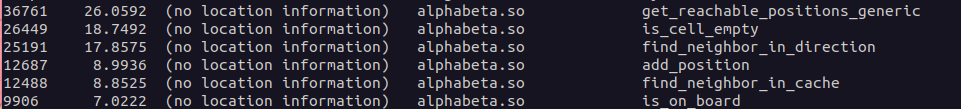
\includegraphics[width=\linewidth]{oprofile_opti}
	\captionsetup{justification=centering}
	\caption{Bilan oprofile d'une exécution d'une partie en utilisant la stratégie \emph{Function Deepening} de notre alphabeta}
\end{figure}

\section{Conclusion}
Pour conclure, nous dirions que le choix de simuler un serveur par un programme \textit{C} qui
charge d'autres librairies dynamiques est relativement étrange. En effet, charger les clients comme des 
librairies dynamiques ouvre la porte à beaucoup de failles, vu que les clients partagent le même espace mémoire que le serveur.
Certaines stratégies malicieuses consisteraient à détecter si nous jouons contre un autre de nos clients, et si cela n'est pas le cas,
on déclenche un crash chez l'autre client, le pénalisant de 10 points sur le ladder. Une faille imparable
serait tout simplement de réserver toute la mémoire disponible, pour empêcher tout appel de \textit{malloc} par l'adversaire.
Cela aurait de très grandes chances de résulter en un \verb|segmentation fault (core dumped)|.

On aurait pu créer un processus par client et serveur, où le serveur et 
les clients communiquent avec un système de \textit{pipes} ou de \textit{socket}.
Cependant, cela explose la complexité du projet sur des points peu intéressants comme 
la transmission de données entre clients et serveurs, ouvrant la porte à multiples bugs obscurs.

\end{document}
